	\pagestyle{euclidthm}

  \def\coordspec{
    \coordinate (A) at (0,0)    ;
    \coordinate (B) at (2,3.5);
    \coordinate (C) at (4,0) ;
    \path (A) -- (B) node[coordinate,pos=0.7] (B') {B'};
    \pgfresetboundingbox
  }
  
 \begin{figure}[h]
   \begin{tikzpicture}[scale=0.8]
     \coordspec
     \tikzsectorabc[fill=yellow]{(C)}{(A)}{(B)}{0.5cm}
     \tikzsectorabc[fill=black]{(B)}{(C)}{(A)}{0.5cm}
     \path[draw=black,thick] (A) -- (B');
     \tikzcorner[yellow][red]{(B')}{(C)}{(A)}
     \tikzcorner[blue][red]{(B)}{(C)}{(A)}
     \tikzcorner[red][black]{(C)}{(A)}{(B')}
     \tikzcorner[white][blue]{(B')}{(B)}{(C)}
     \tikzcorner[black][yellow]{(A)}{(B')}{(C)}
     \path[draw=black,densely dashed,very thick] (B') -- (B);
     \pgfresetboundingbox
     \path (A) -- (B) -- (C) -- cycle;
   \end{tikzpicture}
 \end{figure}
 \def\ABC{%
   \begin{tikzpicture}[scale=0.1]
       \coordspec
       \path[draw=black,thick] (A) -- (B');
       \tikzcorner[blue][red]{(B)}{(C)}{(A)}
       \tikzcorner[red][black]{(C)}{(A)}{(B')}
       \tikzcorner[white][blue]{(B')}{(B)}{(C)}
       \path[draw=black,densely dashed,thick] (B') -- (B);
       \pgfresetboundingbox
       \path (A) -- (B) -- (C) -- cycle;
   \end{tikzpicture}
 }
 \def\ABprimeC{%
   \begin{tikzpicture}[scale=0.1]
       \coordspec
       \tikztriangle[black][yellow][red]{(A)}{(B')}{(C)}
       \pgfresetboundingbox
       \path (A) -- (B') -- (C) -- cycle;
   \end{tikzpicture}
 }
 \def\bac{%
   \begin{tikzpicture}[scale=0.1]
     \coordspec
     \tikzsectorabc[fill=yellow]{(C)}{(A)}{(B)}{0.5cm}
   \end{tikzpicture}
 }
 \def\bca{%
   \begin{tikzpicture}[scale=0.5]
     \coordspec
     \tikzsectorabc[fill=black]{(B)}{(C)}{(A)}{0.5cm}
   \end{tikzpicture}
 }
 \def\ab{%
   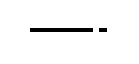
\begin{tikzpicture}[baseline=-0.5ex]
     \draw[ultra thick] (0,0) -- (0.7,0);
     \draw[ultra thick,densely dashed] (0.7,0) -- (1,0);
   \end{tikzpicture}
 }
 \def\bc{%
   \tikzhline[blue]{1cm}
 }
 \def\ac {%
   \tikzhline[red]{1cm}
 }
 \def\abprime{%
   \tikzhline[black]{1cm}
 }
 \def\bprimec{%
   \tikzhline[yellow]{1cm}
 }
  
  \begin{prop}{\lettrine[lines=2]{I}n}
    any triangle (\ABC) if two angles (\bac and \bca) are equal the 
    sides (\ab and \bc) opposite to them are also equal.
  \end{prop}
  \begin{proof}
    For if the sides be not equal, let one of them \ab be greater than 
    the other \bc, and from it cut off $\abprime \equals \bc$ 
    (\refprop{3}), draw \bprimec. 

    Then in \ABprimeC and \ABC, $\abprime \equals \bc$ 
    (\byconstruction) $\bac \equals \bac$ (\byhypothesis) and \ac 
    common, \therefore\ the triangles are equal (\refprop{4}) a part 
    equal to the whole, which is absurd; \therefore\ neither of the 
    sides \ab or \bc is greater than the other, \therefore\ hence they 
    are equal. 
  \end{proof}
